% Options for packages loaded elsewhere
\PassOptionsToPackage{unicode}{hyperref}
\PassOptionsToPackage{hyphens}{url}
%
\documentclass[
]{article}
\usepackage{amsmath,amssymb}
\usepackage{lmodern}
\usepackage{ifxetex,ifluatex}
\ifnum 0\ifxetex 1\fi\ifluatex 1\fi=0 % if pdftex
  \usepackage[T1]{fontenc}
  \usepackage[utf8]{inputenc}
  \usepackage{textcomp} % provide euro and other symbols
\else % if luatex or xetex
  \usepackage{unicode-math}
  \defaultfontfeatures{Scale=MatchLowercase}
  \defaultfontfeatures[\rmfamily]{Ligatures=TeX,Scale=1}
\fi
% Use upquote if available, for straight quotes in verbatim environments
\IfFileExists{upquote.sty}{\usepackage{upquote}}{}
\IfFileExists{microtype.sty}{% use microtype if available
  \usepackage[]{microtype}
  \UseMicrotypeSet[protrusion]{basicmath} % disable protrusion for tt fonts
}{}
\makeatletter
\@ifundefined{KOMAClassName}{% if non-KOMA class
  \IfFileExists{parskip.sty}{%
    \usepackage{parskip}
  }{% else
    \setlength{\parindent}{0pt}
    \setlength{\parskip}{6pt plus 2pt minus 1pt}}
}{% if KOMA class
  \KOMAoptions{parskip=half}}
\makeatother
\usepackage{xcolor}
\IfFileExists{xurl.sty}{\usepackage{xurl}}{} % add URL line breaks if available
\IfFileExists{bookmark.sty}{\usepackage{bookmark}}{\usepackage{hyperref}}
\hypersetup{
  pdftitle={Music Descriptors Supplementary materials},
  pdfauthor={Brendon Mizener},
  hidelinks,
  pdfcreator={LaTeX via pandoc}}
\urlstyle{same} % disable monospaced font for URLs
\usepackage[margin=1in]{geometry}
\usepackage{color}
\usepackage{fancyvrb}
\newcommand{\VerbBar}{|}
\newcommand{\VERB}{\Verb[commandchars=\\\{\}]}
\DefineVerbatimEnvironment{Highlighting}{Verbatim}{commandchars=\\\{\}}
% Add ',fontsize=\small' for more characters per line
\usepackage{framed}
\definecolor{shadecolor}{RGB}{248,248,248}
\newenvironment{Shaded}{\begin{snugshade}}{\end{snugshade}}
\newcommand{\AlertTok}[1]{\textcolor[rgb]{0.94,0.16,0.16}{#1}}
\newcommand{\AnnotationTok}[1]{\textcolor[rgb]{0.56,0.35,0.01}{\textbf{\textit{#1}}}}
\newcommand{\AttributeTok}[1]{\textcolor[rgb]{0.77,0.63,0.00}{#1}}
\newcommand{\BaseNTok}[1]{\textcolor[rgb]{0.00,0.00,0.81}{#1}}
\newcommand{\BuiltInTok}[1]{#1}
\newcommand{\CharTok}[1]{\textcolor[rgb]{0.31,0.60,0.02}{#1}}
\newcommand{\CommentTok}[1]{\textcolor[rgb]{0.56,0.35,0.01}{\textit{#1}}}
\newcommand{\CommentVarTok}[1]{\textcolor[rgb]{0.56,0.35,0.01}{\textbf{\textit{#1}}}}
\newcommand{\ConstantTok}[1]{\textcolor[rgb]{0.00,0.00,0.00}{#1}}
\newcommand{\ControlFlowTok}[1]{\textcolor[rgb]{0.13,0.29,0.53}{\textbf{#1}}}
\newcommand{\DataTypeTok}[1]{\textcolor[rgb]{0.13,0.29,0.53}{#1}}
\newcommand{\DecValTok}[1]{\textcolor[rgb]{0.00,0.00,0.81}{#1}}
\newcommand{\DocumentationTok}[1]{\textcolor[rgb]{0.56,0.35,0.01}{\textbf{\textit{#1}}}}
\newcommand{\ErrorTok}[1]{\textcolor[rgb]{0.64,0.00,0.00}{\textbf{#1}}}
\newcommand{\ExtensionTok}[1]{#1}
\newcommand{\FloatTok}[1]{\textcolor[rgb]{0.00,0.00,0.81}{#1}}
\newcommand{\FunctionTok}[1]{\textcolor[rgb]{0.00,0.00,0.00}{#1}}
\newcommand{\ImportTok}[1]{#1}
\newcommand{\InformationTok}[1]{\textcolor[rgb]{0.56,0.35,0.01}{\textbf{\textit{#1}}}}
\newcommand{\KeywordTok}[1]{\textcolor[rgb]{0.13,0.29,0.53}{\textbf{#1}}}
\newcommand{\NormalTok}[1]{#1}
\newcommand{\OperatorTok}[1]{\textcolor[rgb]{0.81,0.36,0.00}{\textbf{#1}}}
\newcommand{\OtherTok}[1]{\textcolor[rgb]{0.56,0.35,0.01}{#1}}
\newcommand{\PreprocessorTok}[1]{\textcolor[rgb]{0.56,0.35,0.01}{\textit{#1}}}
\newcommand{\RegionMarkerTok}[1]{#1}
\newcommand{\SpecialCharTok}[1]{\textcolor[rgb]{0.00,0.00,0.00}{#1}}
\newcommand{\SpecialStringTok}[1]{\textcolor[rgb]{0.31,0.60,0.02}{#1}}
\newcommand{\StringTok}[1]{\textcolor[rgb]{0.31,0.60,0.02}{#1}}
\newcommand{\VariableTok}[1]{\textcolor[rgb]{0.00,0.00,0.00}{#1}}
\newcommand{\VerbatimStringTok}[1]{\textcolor[rgb]{0.31,0.60,0.02}{#1}}
\newcommand{\WarningTok}[1]{\textcolor[rgb]{0.56,0.35,0.01}{\textbf{\textit{#1}}}}
\usepackage{graphicx}
\makeatletter
\def\maxwidth{\ifdim\Gin@nat@width>\linewidth\linewidth\else\Gin@nat@width\fi}
\def\maxheight{\ifdim\Gin@nat@height>\textheight\textheight\else\Gin@nat@height\fi}
\makeatother
% Scale images if necessary, so that they will not overflow the page
% margins by default, and it is still possible to overwrite the defaults
% using explicit options in \includegraphics[width, height, ...]{}
\setkeys{Gin}{width=\maxwidth,height=\maxheight,keepaspectratio}
% Set default figure placement to htbp
\makeatletter
\def\fps@figure{htbp}
\makeatother
\setlength{\emergencystretch}{3em} % prevent overfull lines
\providecommand{\tightlist}{%
  \setlength{\itemsep}{0pt}\setlength{\parskip}{0pt}}
\setcounter{secnumdepth}{-\maxdimen} % remove section numbering
% Manuscript styling
\usepackage{upgreek}
\usepackage{caption}

\captionsetup{font=singlespacing,justification=justified}

% Table formatting
\usepackage{longtable}
\usepackage{lscape}
% \usepackage[counterclockwise]{rotating}   % Landscape page setup for large tables
\usepackage{multirow}		% Table styling
\usepackage{tabularx}		% Control Column width
\usepackage[flushleft]{threeparttable}	% Allows for three part tables with a specified notes section
\usepackage{threeparttablex}            % Lets threeparttable work with longtable
\usepackage{endfloat}

% Create new environments so endfloat can handle them
% \newenvironment{ltable}
%   {\begin{landscape}\begin{center}\begin{threeparttable}}
%   {\end{threeparttable}\end{center}\end{landscape}}
\newenvironment{lltable}{\begin{landscape}\begin{center}\begin{ThreePartTable}}{\end{ThreePartTable}\end{center}\end{landscape}}

% Enables adjusting longtable caption width to table width
% Solution found at http://golatex.de/longtable-mit-caption-so-breit-wie-die-tabelle-t15767.html
\makeatletter
\newcommand\LastLTentrywidth{1em}
\newlength\longtablewidth
\setlength{\longtablewidth}{1in}
\newcommand{\getlongtablewidth}{\begingroup \ifcsname LT@\roman{LT@tables}\endcsname \global\longtablewidth=0pt \renewcommand{\LT@entry}[2]{\global\advance\longtablewidth by ##2\relax\gdef\LastLTentrywidth{##2}}\@nameuse{LT@\roman{LT@tables}} \fi \endgroup}

% \setlength{\parindent}{0.5in}
% \setlength{\parskip}{0pt plus 0pt minus 0pt}

% \usepackage{etoolbox}
\makeatletter
\patchcmd{\HyOrg@maketitle}
  {\section{\normalfont\normalsize\abstractname}}
  {\section*{\normalfont\normalsize\abstractname}}
  {}{\typeout{Failed to patch abstract.}}
\patchcmd{\HyOrg@maketitle}
  {\section{\protect\normalfont{\@title}}}
  {\section*{\protect\normalfont{\@title}}}
  {}{\typeout{Failed to patch title.}}
\makeatother

\usepackage{deluxetable}
\usepackage{booktabs}
\usepackage{longtable}
\usepackage{array}
\usepackage{multirow}
\usepackage{wrapfig}
\usepackage{float}
\usepackage{colortbl}
\usepackage{pdflscape}
\usepackage{tabu}
\usepackage{threeparttable}
\usepackage{threeparttablex}
\usepackage[normalem]{ulem}
\usepackage{makecell}
\usepackage{xcolor}
\ifluatex
  \usepackage{selnolig}  % disable illegal ligatures
\fi

\title{Music Descriptors Supplementary materials}
\author{Brendon Mizener}
\date{3/29/2021}

\begin{document}
\maketitle

\hypertarget{supplementary-materials-for-experiment-1}{%
\section{Supplementary Materials for Experiment
1}\label{supplementary-materials-for-experiment-1}}

\begin{lltable}
\begin{footnotesize}
\begin{longtable}{p{0.2\textwidth}p{0.2\textwidth}p{0.2\textwidth}p{0.2\textwidth}p{0.2\textwidth}p{0.2\textwidth}}\noalign{\getlongtablewidth\global\LTcapwidth=\longtablewidth}
\caption{\label{tab:qualitiestable}Musical Qualities and the provided survey response options, English.}\\
\toprule[.8pt]
 \multicolumn{1}{c}{Harmonic Material} & \multicolumn{1}{c}{Tempo} & \multicolumn{1}{c}{Meter} & \multicolumn{1}{c}{Density} & \multicolumn{1}{c}{Genre} & \multicolumn{1}{c}{Articulation}\\
 \midrule
      Diatonic: Major & Very slow & Simple Duple & Very sparse & Baroque & Staccato \\
      Diatonic: Minor & Slow & Simple Triple & Moderately sparse & Classical & Marcato \\
      Blues & Moderately Slow & Simple Quadruple  & More sparse than dense & Romantic & Legato\\
      Chromatic & Moderate & Compound Duple & More dense than sparse & Impressionist & Tenuto\\
      Whole tone & Moderately Fast & Compound Triple & Moderately Dense & Modern & Other \\       
      Modal  & Fast & Compound Quadruple & Very Dense & Jazz/Blues & \\
      Quintal/Quartal  & Very Fast & Complex & & Contemporary & \\
      Ambiguous  & & & & Other & \\
      Other  & & & & & \\
\bottomrule\addlinespace[.5em]
 & \multicolumn{1}{c}{Contour} & \multicolumn{1}{c}{Motion} & \multicolumn{1}{c}{Range} & \multicolumn{1}{c}{Dynamics} & \\
 \cmidrule[.5pt]{2-5}
  & Ascending & Conjunct & Narrow & Soft & \\
  & Descending & Disjunct & Moderate & Moderate  & \\
  & Arch & \multirow{2}{0.2\textwidth}{Combination of conjunct and disjunct} & Wide & Loud  & \\
  & Undulating &  & Very Wide & Varied: gradual crescendo &\\
  & Pendulum & \multirow{2}{0.2\textwidth}{I do not think this excerpt has a melody} & \multirow{2}{0.2\textwidth}{I do not think this excerpt has a melody} & \multirow{2}{0.2\textwidth}{Varied: gradual decrescendo} &\\
  & Terrace & & & & \\
  & \multirow{2}{0.2\textwidth}{I do not think this excerpt has a melody} & Other & & \multirow{2}{0.2\textwidth}{Some of each, soft and loud}  &\\
  & & & & & \\
  & Other & & & Other & \\
  
\cmidrule[.75pt]{2-5}
\end{longtable}
\end{footnotesize}
\end{lltable}

\begin{lltable}
\begin{footnotesize}
\begin{longtable}{p{0.2\textwidth}p{0.2\textwidth}p{0.2\textwidth}p{0.2\textwidth}p{0.2\textwidth}p{0.2\textwidth}}\noalign{\getlongtablewidth\global\LTcapwidth=\longtablewidth}
\caption{\label{tab:qualitiestablefr}Musical Qualities and the provided survey response options, French.}\\
\toprule[.8pt]
 \multicolumn{1}{c}{Harmonie} & \multicolumn{1}{c}{Vitesse} & \multicolumn{1}{c}{Mesure} & \multicolumn{1}{c}{Densité} & \multicolumn{1}{c}{Genre} & \multicolumn{1}{c}{Articulation}\\
 \midrule
      Diatonique: majeur & Très lente & Mesure simple, deux temps & Très épurée & Baroque & Staccato \\
      Diatonique: mineur & Lente & Mesure simple, trois temps & Modérément épurée & Classique & Marcato \\
      Gamme Blues & Moyennement lent & Mesure simple, quatre temps & Plutôt épurée que dense & Romantique & Legato\\
      Chromatique & Moyenne & Mesure composée, deux temps & Plutôt dense qu’épurée & Impressioniste & Tenuto\\
      Gamme par ton & Moyennement rapide & Mesure composée, trois temps & Moyennement dense & Moderne & Autre (précisez) \\       
      Modal  & Rapide & Mesure composée, quatre temps & Très dense & Jazz-Blues & \\
      Ambigu  & Très rapide & Mesure complexe & & Contemporarain & \\
      \multirow{2}{0.2\textwidth}{Je ne pense pas que cet extrait ait une mélodie}  & & & & Autre (précisez) & \\
      Autre (précisez)  & & & & & \\
\bottomrule\addlinespace[.5em]
 & \multicolumn{1}{c}{Contour} & \multicolumn{1}{c}{Mouvement} & \multicolumn{1}{c}{Ambitus} & \multicolumn{1}{c}{Dynamiques} & \\
 \cmidrule[.5pt]{2-5}
  & Ascendant & Conjoint & Ambitus resserré & Doux & \\
  & Descendant & Disjoint & Ambitus modéré & Moyen  & \\
  & Forme en arche & \multirow{2}{0.2\textwidth}{Une combinaison de conjoint et disjoint} & Ambitus grand & Fort  & \\
  & Petites vagues successives &  & Ambitus très grand & Varié : crescendo progressif &\\
  & Grandes vagues successives & \multirow{2}{0.2\textwidth}{Je ne pense pas que cet extrait ait une mélodie} & \multirow{2}{0.2\textwidth}{Je ne pense pas que cet extrait ait une mélodie} & \multirow{2}{0.2\textwidth}{Varié : decrescendo progressif} &\\
  & Plusieurs phases descendantes successives & & & & \\
  & \multirow{2}{0.2\textwidth}{Je ne pense pas que cet extrait ait une mélodie} & Autre (précisez) & & \multirow{2}{0.2\textwidth}{Un peu des deux: doux et fort}  &\\
  & & & & & \\
  & Autre (précisez) & & & Autre (précisez) & \\
  
\cmidrule[.75pt]{2-5}
\end{longtable}
\end{footnotesize}
\end{lltable}

\begin{center}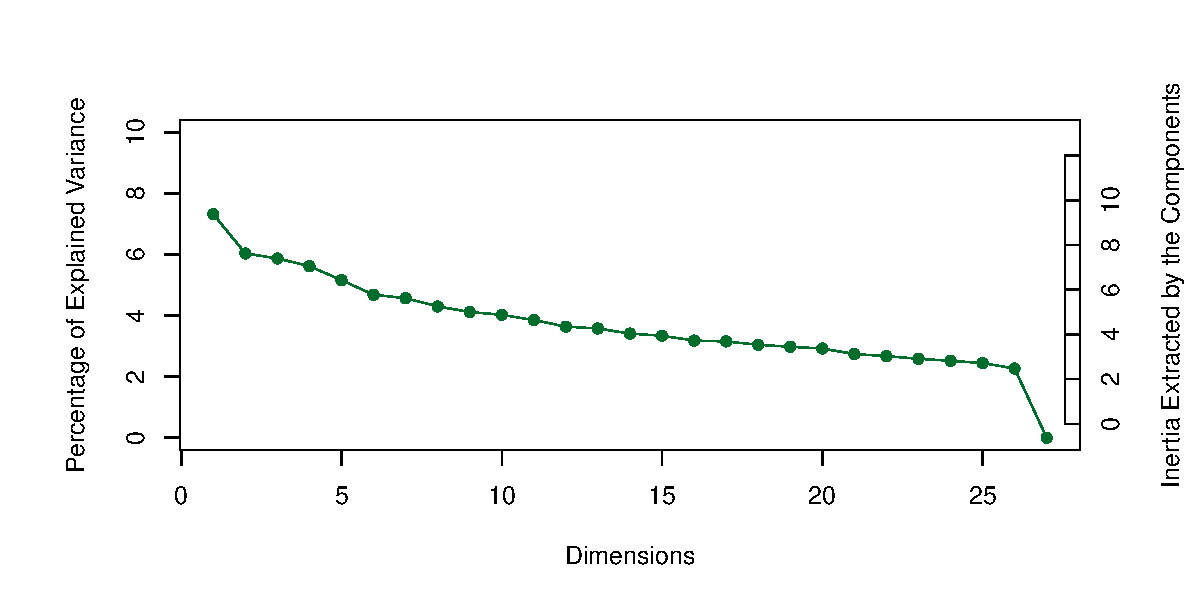
\includegraphics{MusDes_Supplementary_files/figure-latex/screeRV-1} \end{center}

\begin{Shaded}
\begin{Highlighting}[]
\NormalTok{n.ellipse }\OtherTok{\textless{}{-}} \FunctionTok{MakeCIEllipses}\NormalTok{(BootCube.N}\SpecialCharTok{$}\NormalTok{BootCube[,}\DecValTok{1}\SpecialCharTok{:}\DecValTok{2}\NormalTok{,], }
                            \AttributeTok{names.of.factors =} \FunctionTok{c}\NormalTok{(}\StringTok{"Dimension 1"}\NormalTok{,}\StringTok{"Dimension 2"}\NormalTok{),}
                            \AttributeTok{col =} \FunctionTok{c}\NormalTok{(col4AM, col4FR))}
\NormalTok{g.ellipse }\OtherTok{\textless{}{-}} \FunctionTok{MakeCIEllipses}\NormalTok{(BootCube.G}\SpecialCharTok{$}\NormalTok{BootCube[,}\DecValTok{1}\SpecialCharTok{:}\DecValTok{2}\NormalTok{,], }
                            \AttributeTok{names.of.factors =} \FunctionTok{c}\NormalTok{(}\StringTok{"Dimension 1"}\NormalTok{,}\StringTok{"Dimension 2"}\NormalTok{),}
                            \AttributeTok{col =} \FunctionTok{c}\NormalTok{(col4M, col4F))}
\end{Highlighting}
\end{Shaded}

\begin{Shaded}
\begin{Highlighting}[]
\FunctionTok{grid.arrange}\NormalTok{(}\FunctionTok{as.grob}\NormalTok{(a.}\FloatTok{01.}\NormalTok{map4part), }
             \FunctionTok{as.grob}\NormalTok{(a.}\FloatTok{02.}\NormalTok{map4part), }\AttributeTok{ncol =} \DecValTok{2}\NormalTok{,}
             \AttributeTok{top =} \FunctionTok{textGrob}\NormalTok{(}\StringTok{"Factor Scores for Expert Ratings"}\NormalTok{, }
                            \AttributeTok{gp =} \FunctionTok{gpar}\NormalTok{(}\AttributeTok{fontsize =} \DecValTok{18}\NormalTok{, }\AttributeTok{font =} \DecValTok{3}\NormalTok{)))}
\end{Highlighting}
\end{Shaded}

\begin{center}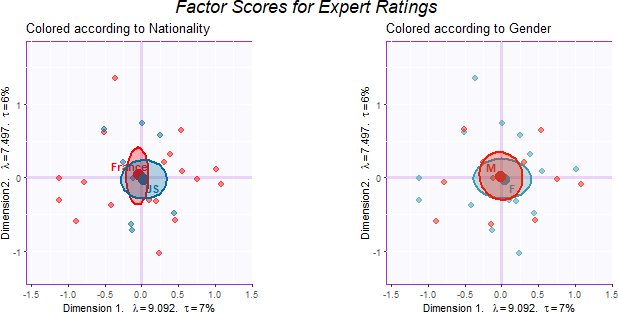
\includegraphics{MusDes_Supplementary_files/figure-latex/printRVbydesign-1} \end{center}

\begin{center}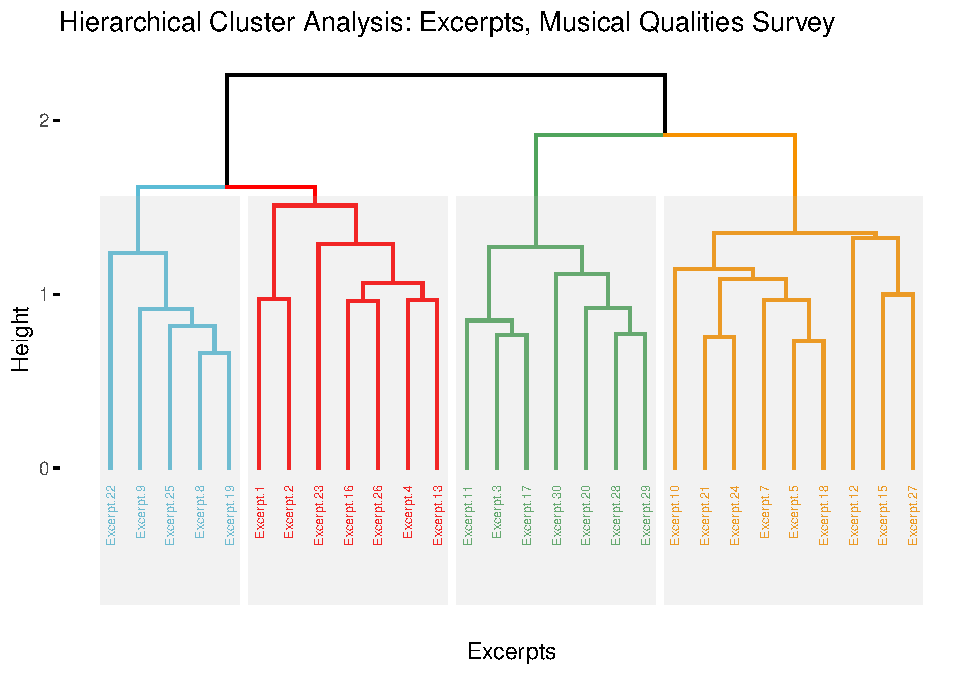
\includegraphics{MusDes_Supplementary_files/figure-latex/HCA-1} \end{center}

\begin{center}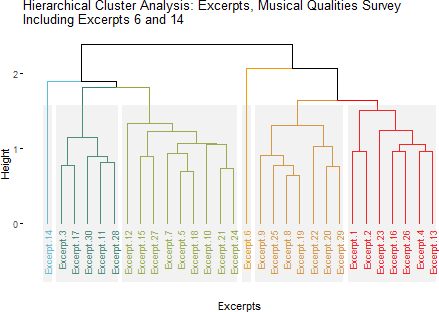
\includegraphics{MusDes_Supplementary_files/figure-latex/HCAW6-1} \end{center}

\begin{center}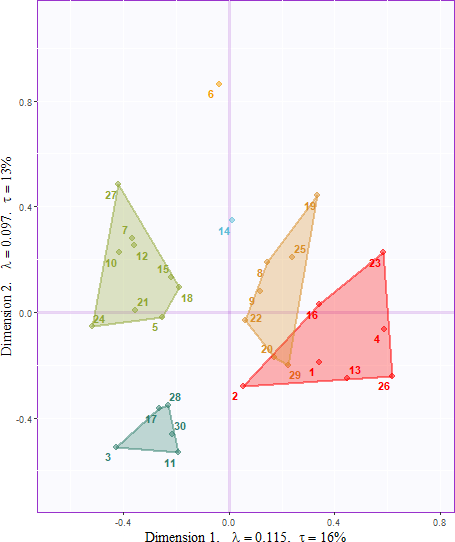
\includegraphics{MusDes_Supplementary_files/figure-latex/excerptsmaps23-1} \end{center}

\begin{center}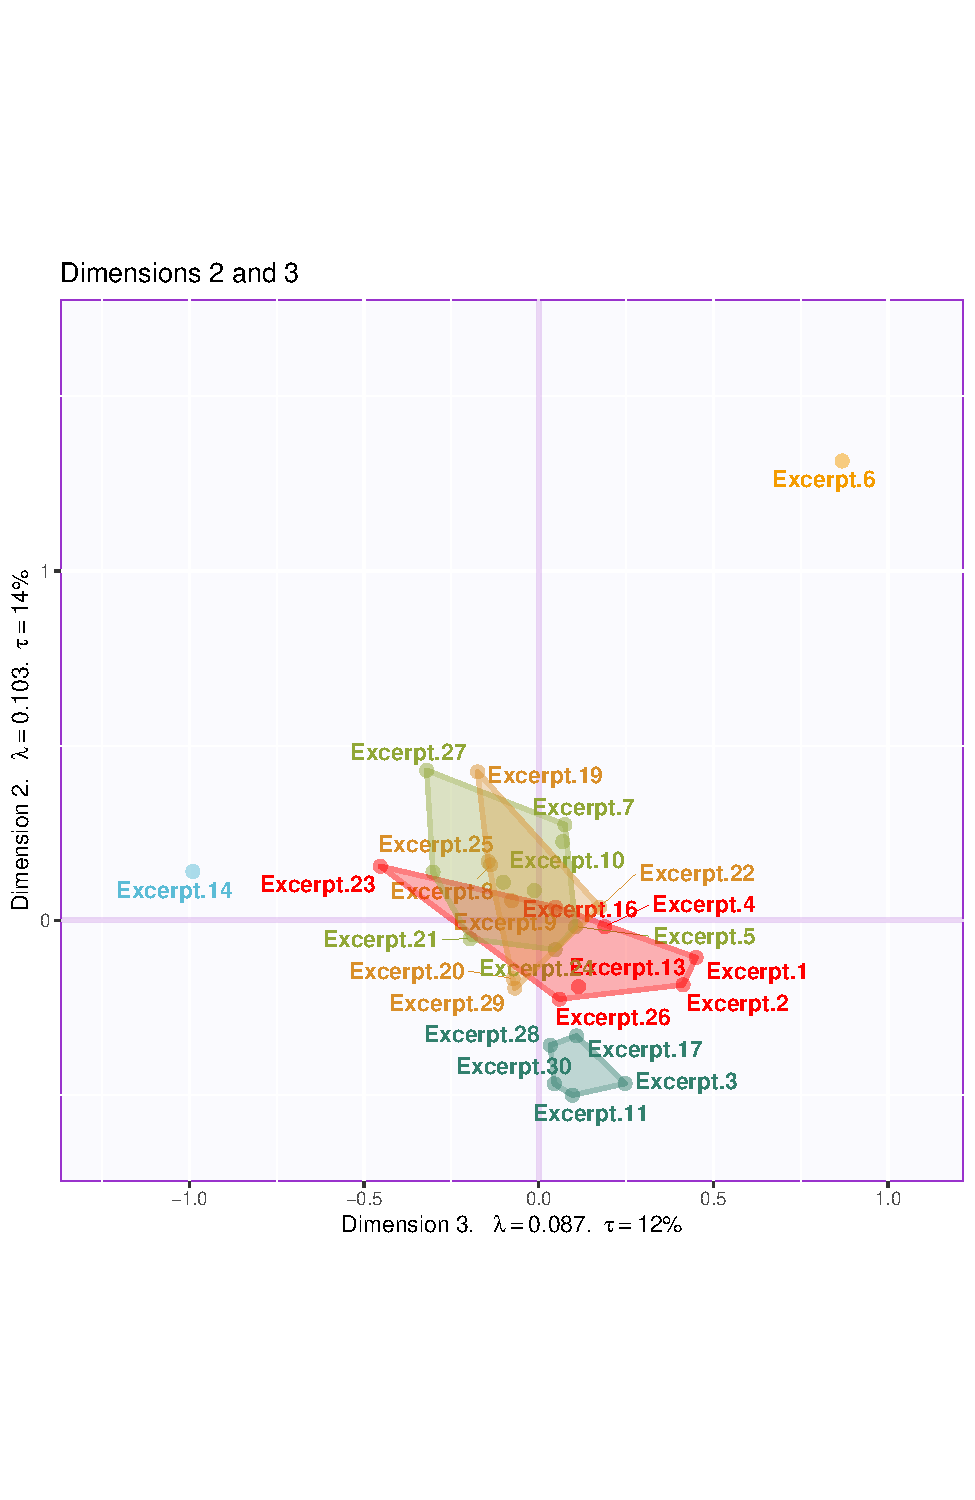
\includegraphics{MusDes_Supplementary_files/figure-latex/excerptsmaps23-2} \end{center}

\begin{Shaded}
\begin{Highlighting}[]
\NormalTok{axisone }\OtherTok{\textless{}{-}} \DecValTok{1}
\NormalTok{axistwo }\OtherTok{\textless{}{-}} \DecValTok{2}


\NormalTok{mustau }\OtherTok{\textless{}{-}}\NormalTok{ dimcares.inf}\SpecialCharTok{$}\NormalTok{Fixed.Data}\SpecialCharTok{$}\NormalTok{ExPosition.Data}\SpecialCharTok{$}\NormalTok{pdq}\SpecialCharTok{$}\NormalTok{tau}
\NormalTok{muslam }\OtherTok{\textless{}{-}}\NormalTok{ dimcares.inf}\SpecialCharTok{$}\NormalTok{Fixed.Data}\SpecialCharTok{$}\NormalTok{ExPosition.Data}\SpecialCharTok{$}\NormalTok{pdq}\SpecialCharTok{$}\NormalTok{eigs}


\NormalTok{labelsforexcerpts }\OtherTok{\textless{}{-}} \FunctionTok{createxyLabels.gen}\NormalTok{(axisone, axistwo,}\AttributeTok{lambda =}\NormalTok{ muslam, }\AttributeTok{tau =}\NormalTok{ mustau)}

\NormalTok{Basemap.cols }\OtherTok{\textless{}{-}} \FunctionTok{createFactorMap}\NormalTok{(}\AttributeTok{X =}\NormalTok{ FJs,}
                                    \AttributeTok{axis1 =}\NormalTok{ axisone,}
                                    \AttributeTok{axis2 =}\NormalTok{ axistwo, }
                                    \AttributeTok{col.points =}\NormalTok{ col4cols,}
\CommentTok{\#                                    constraints = Basemap.excerpts$constraints,}
                                    \AttributeTok{title =} \StringTok{"Column Factor Scores }\SpecialCharTok{\textbackslash{}n}\StringTok{Colored according to dimension group"}\NormalTok{,}
                                    \AttributeTok{display.points =}\NormalTok{ T,}
                                    \AttributeTok{pch =} \DecValTok{19}\NormalTok{, }\AttributeTok{cex =} \DecValTok{4}\NormalTok{,}
                                    \AttributeTok{display.labels =}\NormalTok{ T,}
                                    \AttributeTok{col.labels =}\NormalTok{ col4cols,}
                                    \AttributeTok{text.cex =} \DecValTok{4}\NormalTok{, }\AttributeTok{font.face =} \StringTok{"bold"}\NormalTok{,}
                                    \AttributeTok{font.family =} \StringTok{"sans"}\NormalTok{,}
                                    \AttributeTok{col.axes =} \StringTok{"darkorchid"}\NormalTok{,}
                                    \AttributeTok{alpha.axes =} \FloatTok{0.2}\NormalTok{,}
                                    \AttributeTok{width.axes =} \FloatTok{1.1}\NormalTok{,}
                                    \AttributeTok{col.background =} \FunctionTok{adjustcolor}\NormalTok{(}\StringTok{"lavender"}\NormalTok{,}
                                                       \AttributeTok{alpha.f =} \FloatTok{0.2}\NormalTok{),}
                                    \AttributeTok{force =} \DecValTok{1}\NormalTok{, }\AttributeTok{segment.size =} \DecValTok{3}
\NormalTok{                                    )}
                                    

\NormalTok{mus}\FloatTok{.007} \OtherTok{\textless{}{-}}\NormalTok{ Basemap.cols}\SpecialCharTok{$}\NormalTok{zeMap\_background }\SpecialCharTok{+}\NormalTok{ labelsforexcerpts }\SpecialCharTok{+}\NormalTok{ Basemap.cols}\SpecialCharTok{$}\NormalTok{zeMap\_dots}
\NormalTok{mus}\FloatTok{.008} \OtherTok{\textless{}{-}}\NormalTok{ Basemap.cols}\SpecialCharTok{$}\NormalTok{zeMap\_background }\SpecialCharTok{+}\NormalTok{ labelsforexcerpts }\SpecialCharTok{+}\NormalTok{ Basemap.cols}\SpecialCharTok{$}\NormalTok{zeMap\_text}
\NormalTok{mus}\FloatTok{.009} \OtherTok{\textless{}{-}}\NormalTok{ Basemap.cols}\SpecialCharTok{$}\NormalTok{zeMap }\SpecialCharTok{+}\NormalTok{ labelsforexcerpts}

\FunctionTok{print}\NormalTok{(mus}\FloatTok{.009}\NormalTok{)}
\end{Highlighting}
\end{Shaded}

\begin{center}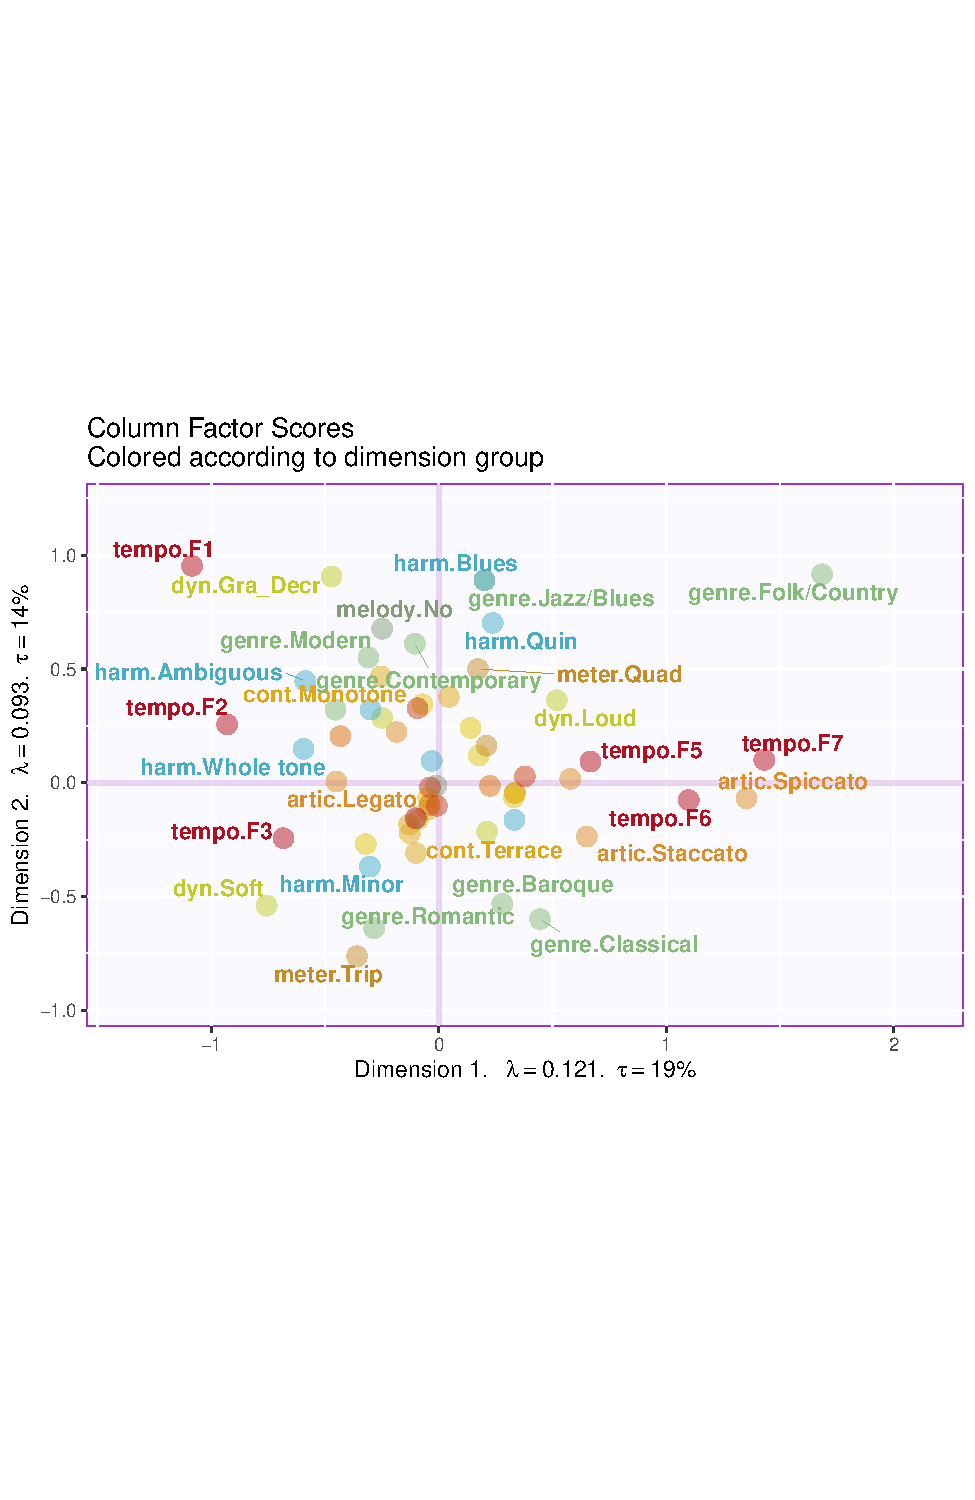
\includegraphics[width=1\linewidth]{MusDes_Supplementary_files/figure-latex/colmaps-1} \end{center}

\begin{Shaded}
\begin{Highlighting}[]
\CommentTok{\# This was originally initialized as something else. Instead of changing each}
\CommentTok{\# instance, I\textquotesingle{}m just changing this one.}
\NormalTok{FJ.all }\OtherTok{\textless{}{-}}\NormalTok{ FJs}
\CommentTok{\#Initialize an empty list}
\NormalTok{FJ.split }\OtherTok{\textless{}{-}} \FunctionTok{vector}\NormalTok{(}\AttributeTok{mode =} \StringTok{"list"}\NormalTok{, }\AttributeTok{length =} \FunctionTok{length}\NormalTok{(numberofdims))}

\CommentTok{\# Name the elements of the list with the names of each group of musical dimensions}
\FunctionTok{names}\NormalTok{(FJ.split) }\OtherTok{\textless{}{-}} \FunctionTok{names}\NormalTok{(numberofdims)}

\CommentTok{\# This loop puts the factor scores for each group of musical dimensions }
\CommentTok{\# in each element of the list}
\ControlFlowTok{for}\NormalTok{ (i }\ControlFlowTok{in} \DecValTok{1}\SpecialCharTok{:}\FunctionTok{length}\NormalTok{(numberofdims))\{}
\NormalTok{    FJ.split[[i]] }\OtherTok{=}\NormalTok{ FJ.all[}\FunctionTok{which}\NormalTok{(}\FunctionTok{stri\_startswith}\NormalTok{(}\FunctionTok{rownames}\NormalTok{(FJ.all), }
                                                 \AttributeTok{coll =} \FunctionTok{names}\NormalTok{(numberofdims)[i])), ]}
\NormalTok{    \}}

\CommentTok{\# We also need to do the same for the constraints}
\NormalTok{FJ.constraints }\OtherTok{\textless{}{-}} \FunctionTok{vector}\NormalTok{(}\AttributeTok{mode =} \StringTok{"list"}\NormalTok{, }\AttributeTok{length =} \FunctionTok{length}\NormalTok{(numberofdims))}
\FunctionTok{names}\NormalTok{(FJ.constraints) }\OtherTok{=} \FunctionTok{names}\NormalTok{(numberofdims)}
\NormalTok{axisone }\OtherTok{\textless{}{-}} \DecValTok{1}
\NormalTok{axistwo }\OtherTok{\textless{}{-}} \DecValTok{2}

\ControlFlowTok{for}\NormalTok{ (i }\ControlFlowTok{in} \DecValTok{1}\SpecialCharTok{:}\FunctionTok{length}\NormalTok{(numberofdims))\{}
    
\NormalTok{  FJ.constraints[[i]] }\OtherTok{\textless{}{-}} \FunctionTok{minmaxHelper}\NormalTok{(FJ.split[[i]], }
                                      \AttributeTok{axis1 =}\NormalTok{ axisone, }\AttributeTok{axis2 =}\NormalTok{ axistwo)}
\NormalTok{\}}

\CommentTok{\# And finally we need to create a list for the actual maps}
\NormalTok{FJ.maps }\OtherTok{\textless{}{-}} \FunctionTok{vector}\NormalTok{(}\AttributeTok{mode =} \StringTok{"list"}\NormalTok{, }\AttributeTok{length =} \FunctionTok{length}\NormalTok{(numberofdims))}
\FunctionTok{names}\NormalTok{(FJ.maps) }\OtherTok{=} \FunctionTok{names}\NormalTok{(numberofdims)}
\CommentTok{\# This loop uses the three lists we\textquotesingle{}ve created to create a set of maps, with one}
\CommentTok{\# for each group of factor scores.}


\ControlFlowTok{for}\NormalTok{ (i }\ControlFlowTok{in} \DecValTok{1}\SpecialCharTok{:}\FunctionTok{length}\NormalTok{(numberofdims))\{}
  
\NormalTok{  FJ.maps[[i]] }\OtherTok{\textless{}{-}} \FunctionTok{createFactorMap}\NormalTok{(FJ.split[[i]],}
                                  \AttributeTok{axis1 =}\NormalTok{ axisone, }\AttributeTok{axis2 =}\NormalTok{ axistwo,}
                                  \AttributeTok{constraints =}\NormalTok{ Basemap.cols}\SpecialCharTok{$}\NormalTok{constraints,}
                                  \AttributeTok{col.points =} \FunctionTok{unique}\NormalTok{(col4cols)[i],}
                                    \AttributeTok{display.points =}\NormalTok{ T,}
                                    \AttributeTok{pch =} \DecValTok{19}\NormalTok{, }\AttributeTok{cex =} \FloatTok{2.5}\NormalTok{,}
                                    \AttributeTok{display.labels =}\NormalTok{ T,}
                                    \AttributeTok{col.labels =} \FunctionTok{unique}\NormalTok{(col4cols)[i],}
                                    \AttributeTok{text.cex =} \FloatTok{2.5}\NormalTok{, }\AttributeTok{font.face =} \StringTok{"bold"}\NormalTok{,}
                                    \AttributeTok{font.family =} \StringTok{"sans"}\NormalTok{,}
                                    \AttributeTok{col.axes =} \StringTok{"darkorchid"}\NormalTok{,}
                                    \AttributeTok{alpha.axes =} \FloatTok{0.2}\NormalTok{,}
                                    \AttributeTok{width.axes =} \FloatTok{1.1}\NormalTok{,}
                                    \AttributeTok{col.background =} \FunctionTok{adjustcolor}\NormalTok{(}\StringTok{"lavender"}\NormalTok{,}
                                                       \AttributeTok{alpha.f =} \FloatTok{0.2}\NormalTok{),}
                                    \AttributeTok{force =} \DecValTok{1}\NormalTok{, }\AttributeTok{segment.size =} \DecValTok{3}
\NormalTok{                                    )}
  \FunctionTok{print}\NormalTok{(FJ.maps[[i]]}\SpecialCharTok{$}\NormalTok{zeMap }\SpecialCharTok{+}\NormalTok{ labelsforexcerpts)}
\NormalTok{\}}
\end{Highlighting}
\end{Shaded}

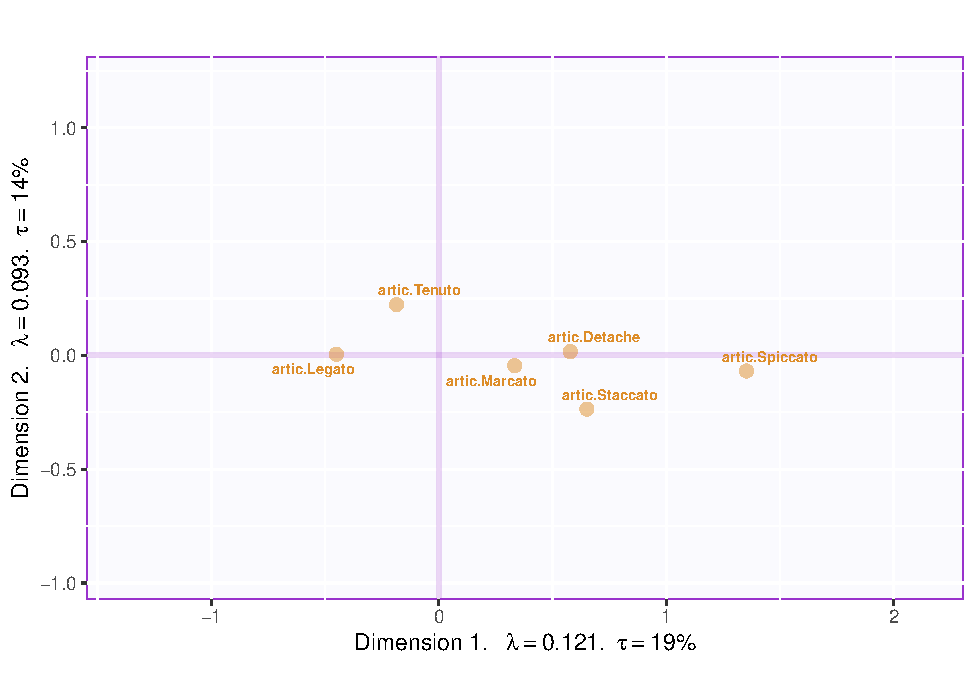
\includegraphics[width=0.5\linewidth]{MusDes_Supplementary_files/figure-latex/morecolmaps-1}
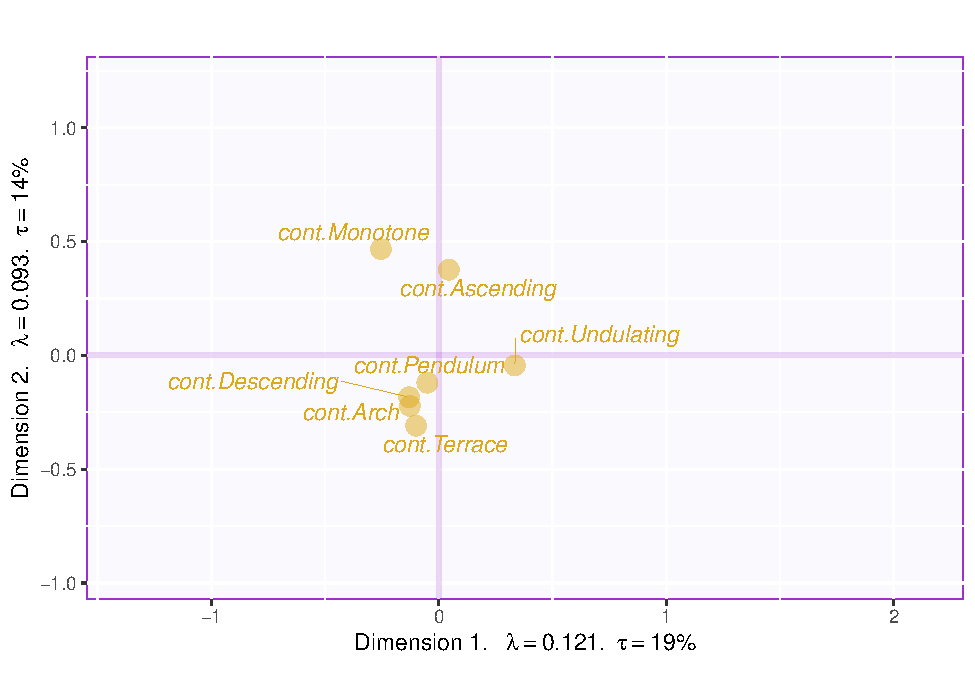
\includegraphics[width=0.5\linewidth]{MusDes_Supplementary_files/figure-latex/morecolmaps-2}
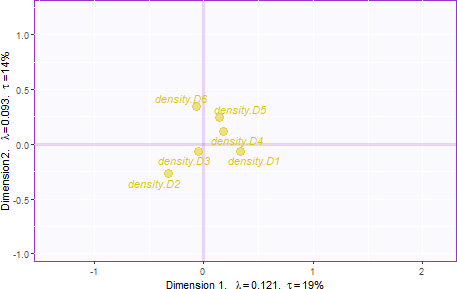
\includegraphics[width=0.5\linewidth]{MusDes_Supplementary_files/figure-latex/morecolmaps-3}
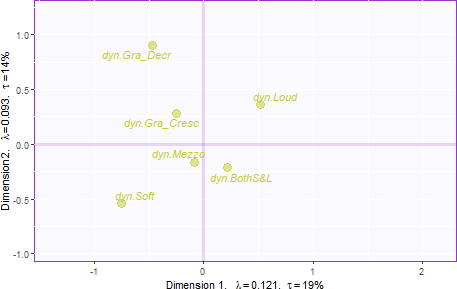
\includegraphics[width=0.5\linewidth]{MusDes_Supplementary_files/figure-latex/morecolmaps-4}
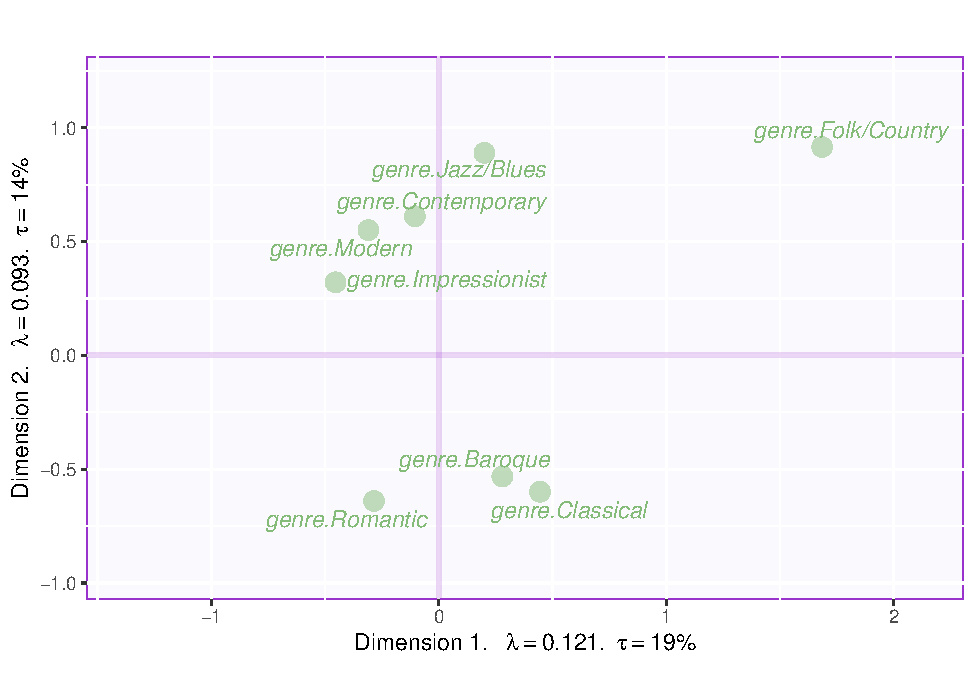
\includegraphics[width=0.5\linewidth]{MusDes_Supplementary_files/figure-latex/morecolmaps-5}
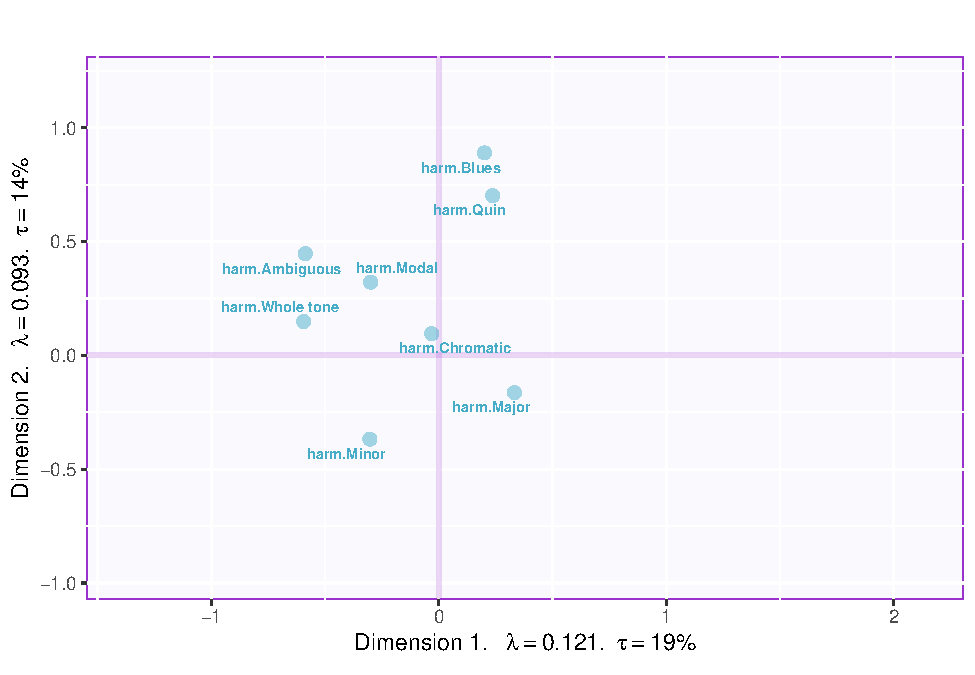
\includegraphics[width=0.5\linewidth]{MusDes_Supplementary_files/figure-latex/morecolmaps-6}
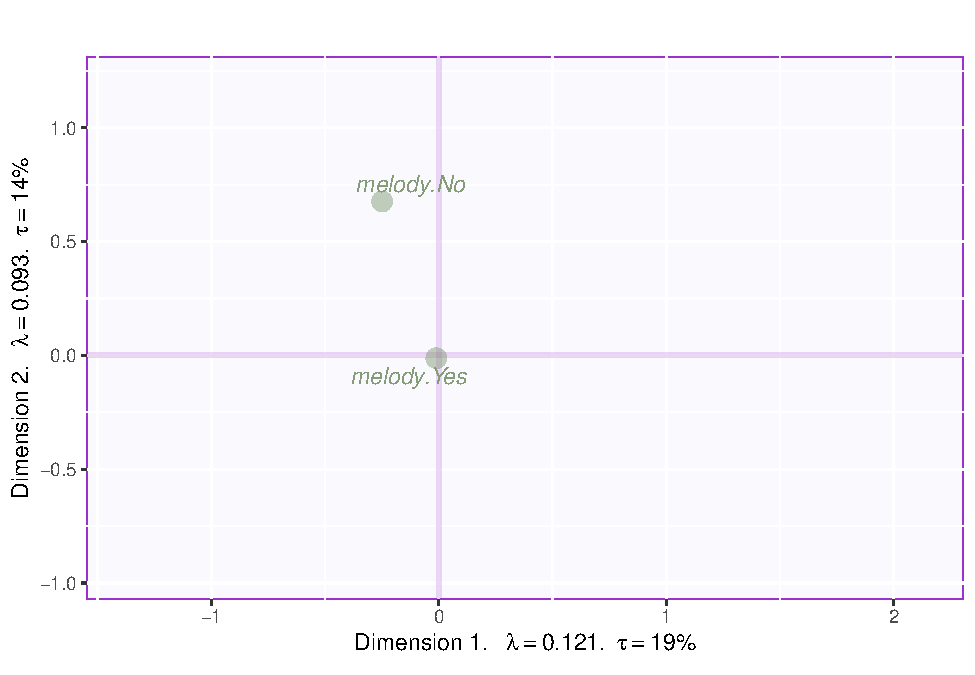
\includegraphics[width=0.5\linewidth]{MusDes_Supplementary_files/figure-latex/morecolmaps-7}
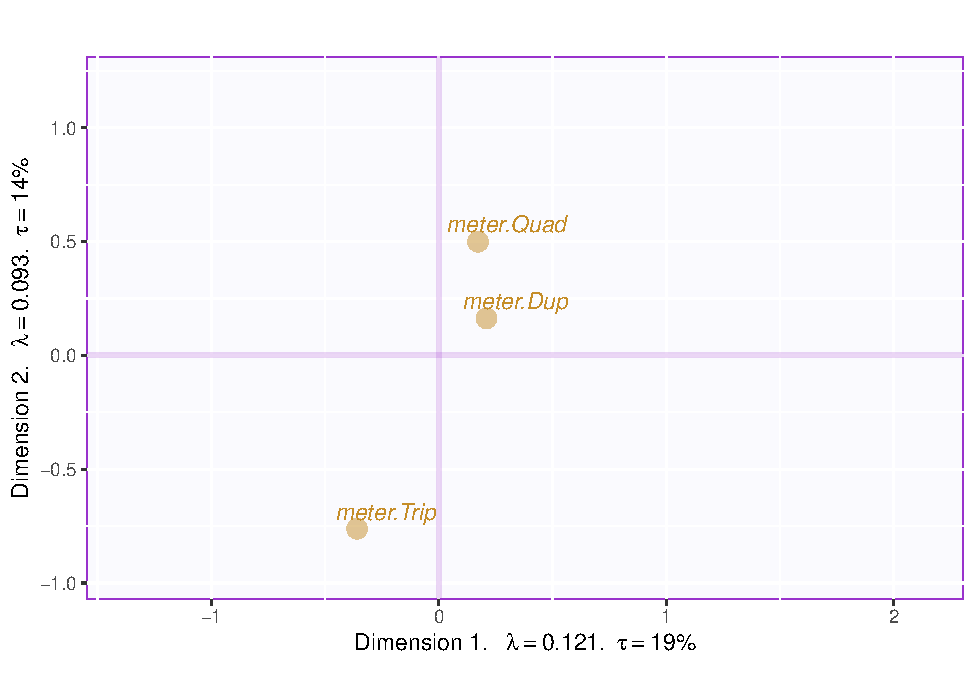
\includegraphics[width=0.5\linewidth]{MusDes_Supplementary_files/figure-latex/morecolmaps-8}
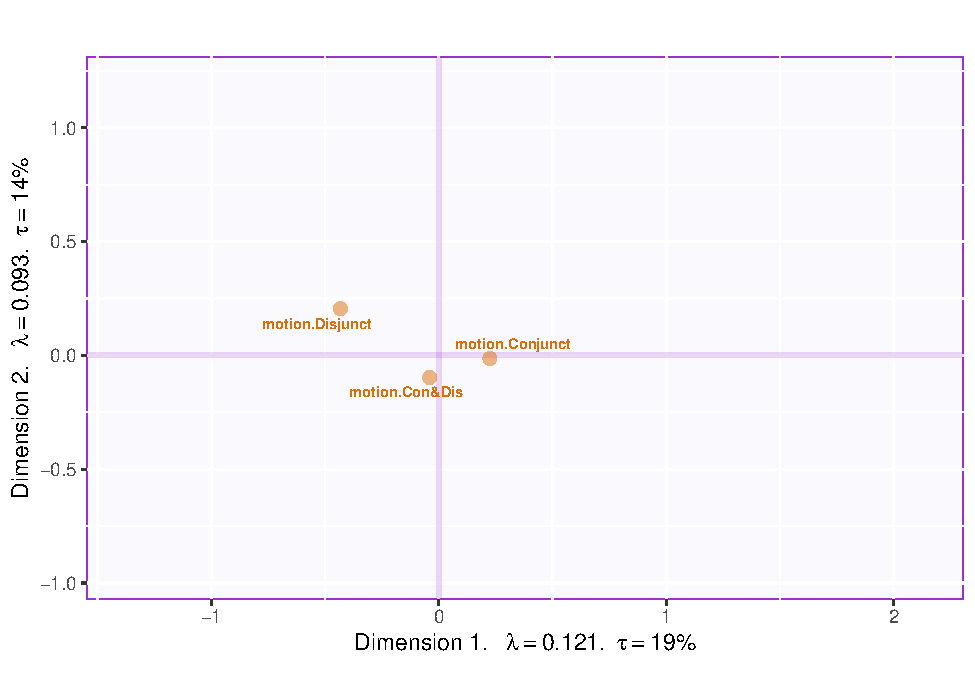
\includegraphics[width=0.5\linewidth]{MusDes_Supplementary_files/figure-latex/morecolmaps-9}
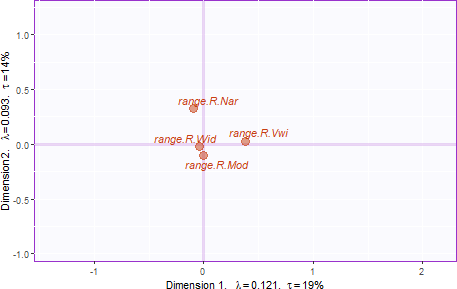
\includegraphics[width=0.5\linewidth]{MusDes_Supplementary_files/figure-latex/morecolmaps-10}
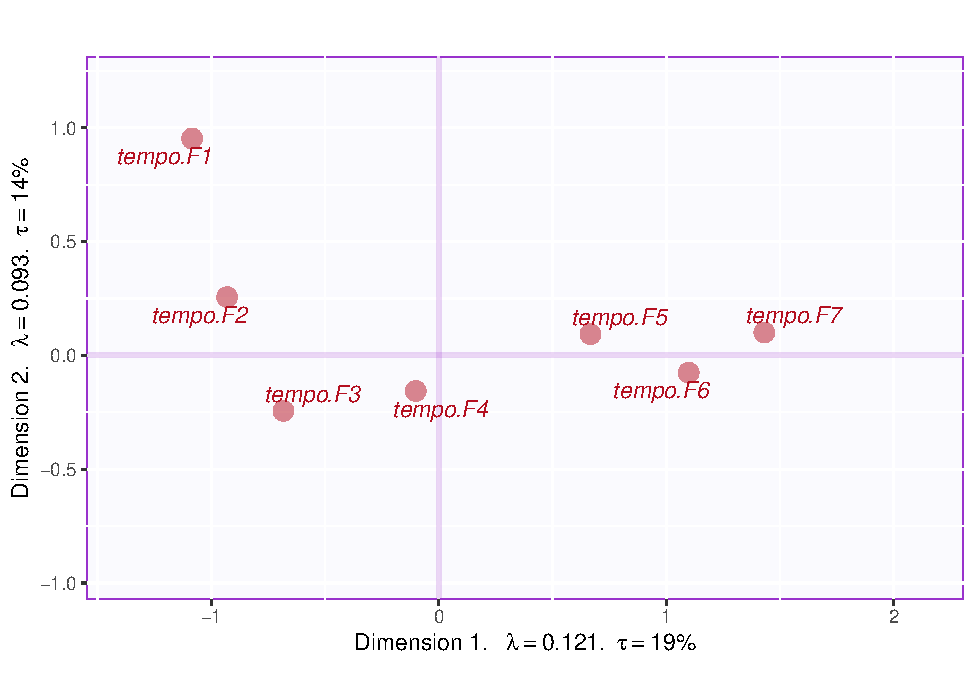
\includegraphics[width=0.5\linewidth]{MusDes_Supplementary_files/figure-latex/morecolmaps-11}

\begin{center}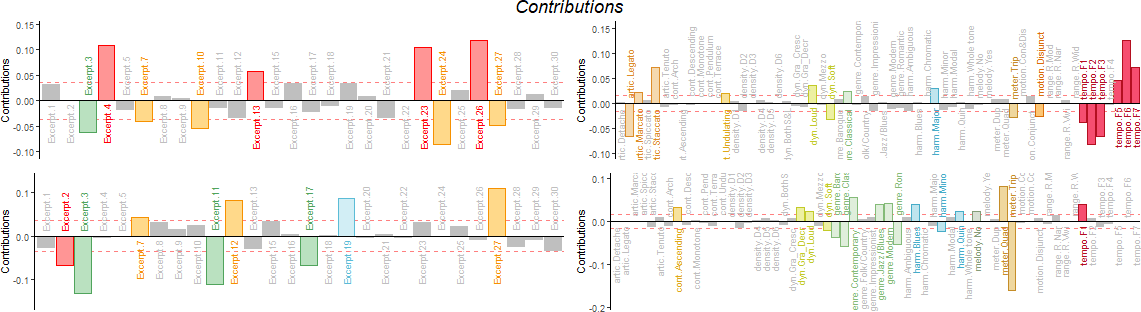
\includegraphics{MusDes_Supplementary_files/figure-latex/contributionsqsup-1} \end{center}

\hypertarget{supplementary-materials-for-experiment-2}{%
\section{Supplementary Materials for Experiment
2}\label{supplementary-materials-for-experiment-2}}

\begin{table}[h]

\begin{center}
\begin{threeparttable}

\caption{\label{tab:adjtable}CATA Adjectives}

\begin{tabular}{ll}
\toprule
English & \multicolumn{1}{c}{French}\\
\midrule
Slow & Lent\\
Fast & Rapide\\
Dense & Bavard\\
Sparse & Epure\\
Complex & Complexe\\
Transparent & Transparent\\
Light & Clair\\
Dark & Sombre\\
Bright & Brillant\\
Dull & Terne\\
Soft & Doux\\
Strong & Fort\\
Mysterious & Mysterieux\\
Melancholy & Melancolique\\
Incisive & Incisif\\
Round & Tendre\\
Aggressive & Agressif\\
Weak & Faible\\
Strong & Puissant\\
Warm & Chaleureux\\
Solemn & Solennel\\
Valiant & Vaillant\\
Sad & Triste\\
Happy & Joyeux\\
Dancing & Dansant\\
Disturbing & Inquietant\\
Exotic & Exotique\\
Colorful & Colore\\
Varied & Changeant\\
Monotonous & Monotone\\
Long & Long\\
Short & Court\\
Surprising & Surprenant\\
\bottomrule
\end{tabular}

\end{threeparttable}
\end{center}

\end{table}

\begin{center}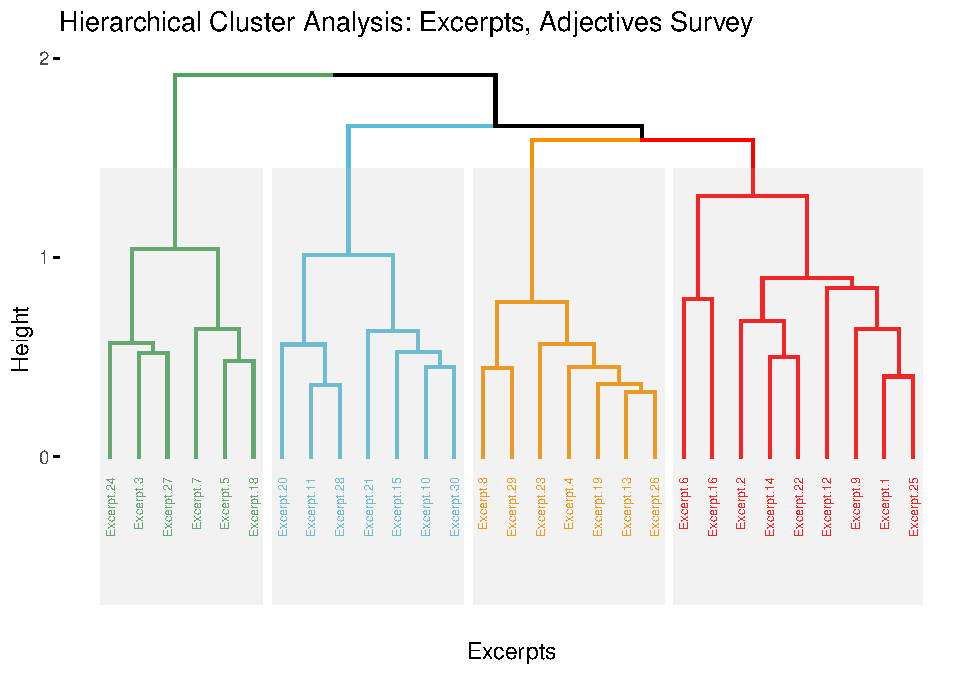
\includegraphics{MusDes_Supplementary_files/figure-latex/HCA.adj-1} \end{center}

\begin{center}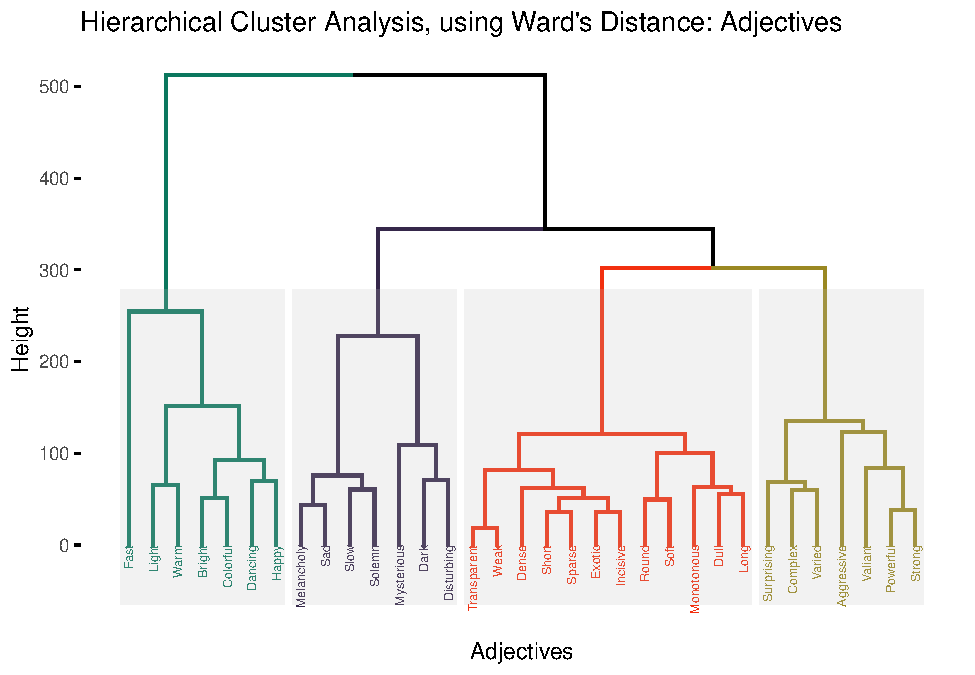
\includegraphics{MusDes_Supplementary_files/figure-latex/HCA4words-1} \end{center}

\begin{center}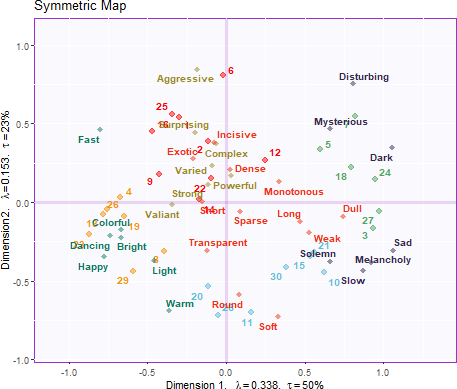
\includegraphics[width=1\linewidth]{MusDes_Supplementary_files/figure-latex/symmetricmap-1} 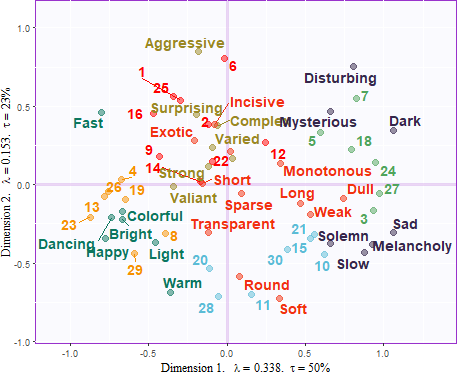
\includegraphics[width=1\linewidth]{MusDes_Supplementary_files/figure-latex/symmetricmap-2} \end{center}

\begin{center}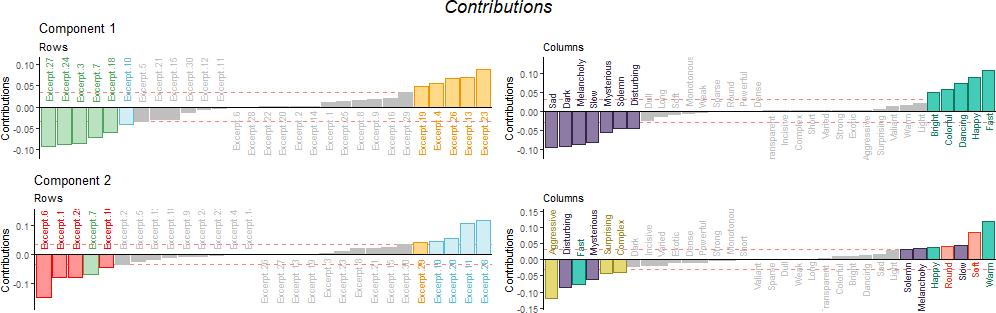
\includegraphics{MusDes_Supplementary_files/figure-latex/thecons-1} \end{center}

\hypertarget{supplementary-materials-for-experiment-3}{%
\section{Supplementary materials for Experiment
3}\label{supplementary-materials-for-experiment-3}}

\begin{center}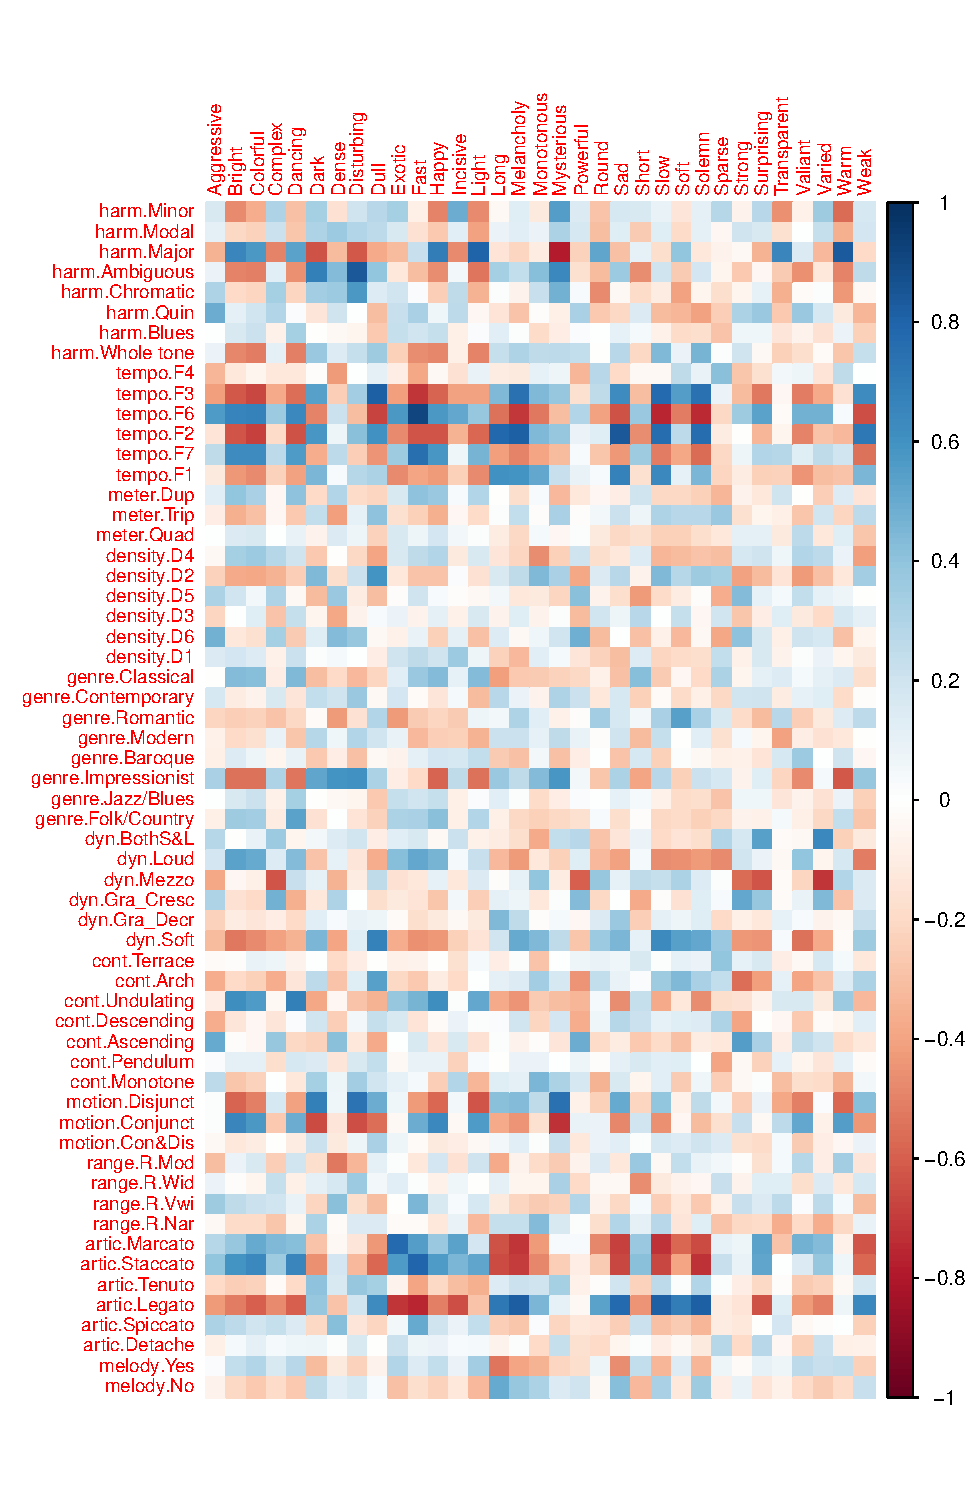
\includegraphics{MusDes_Supplementary_files/figure-latex/covariance.mat-1} \end{center}

\begin{center}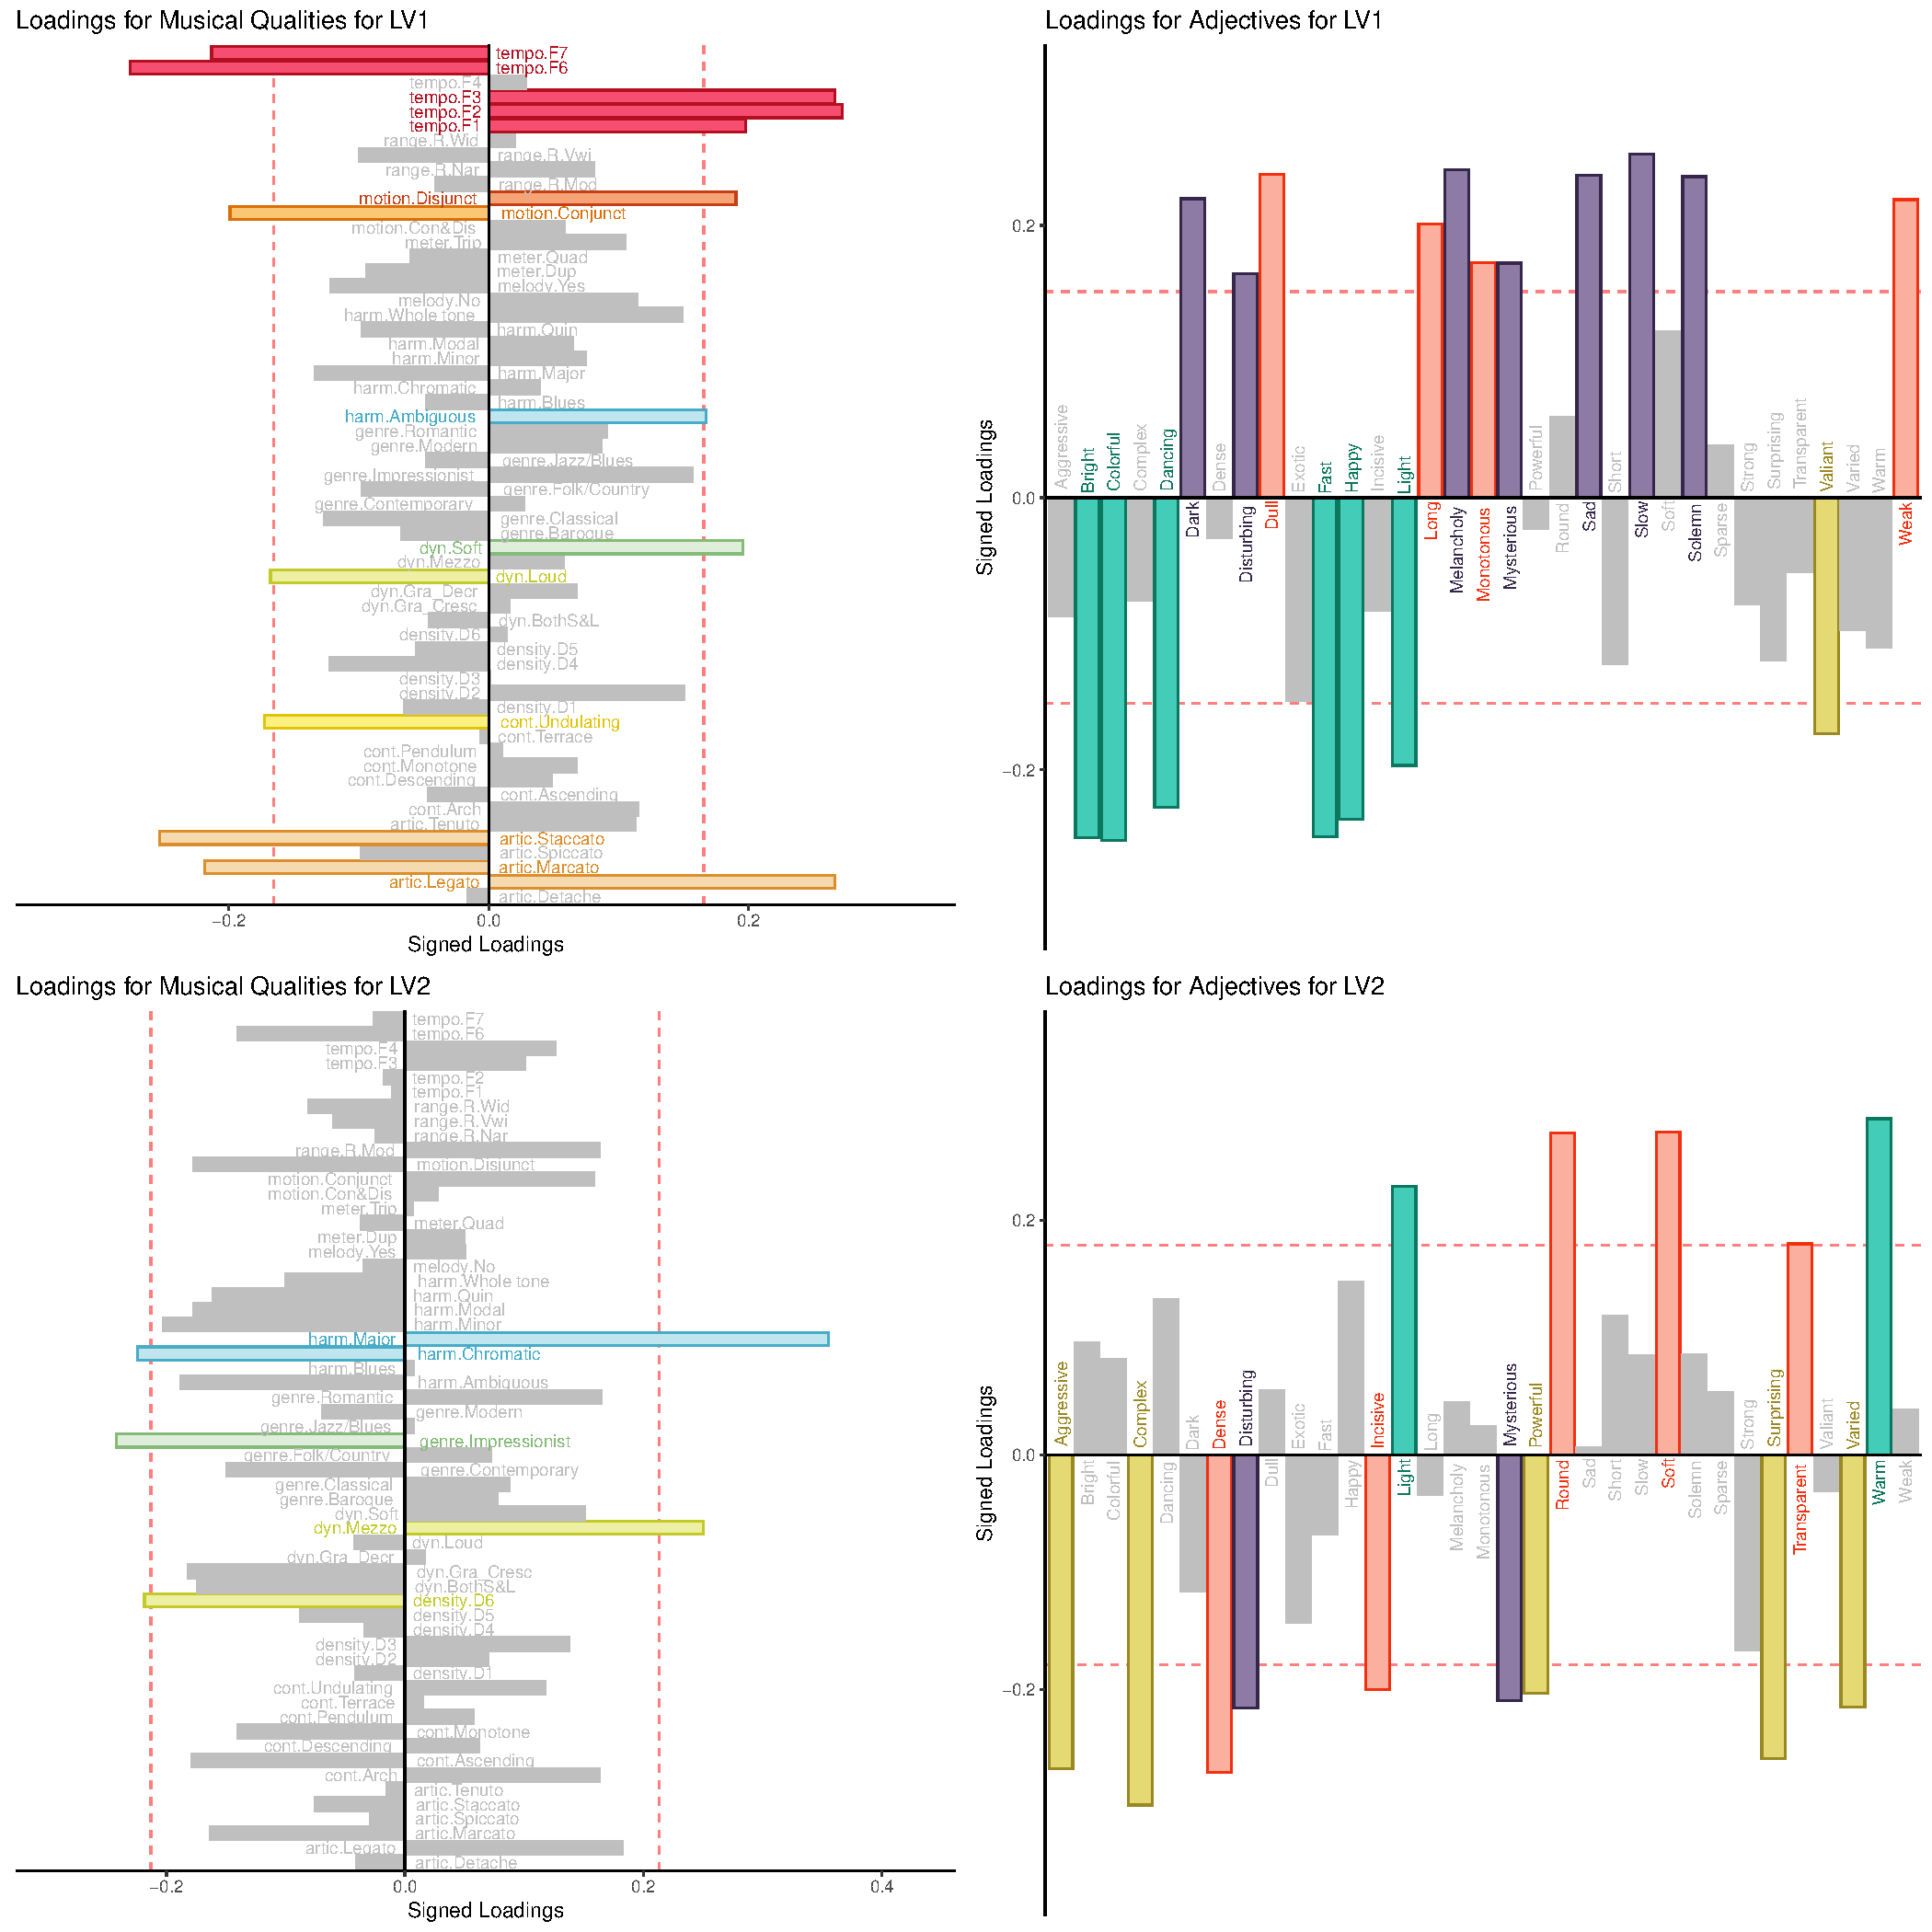
\includegraphics{MusDes_Supplementary_files/figure-latex/loadingbarplotplscsup-1} \end{center}

\end{document}
